\clearpage
\addcontentsline{toc}{section}{\numberline{}Our Workspaces}
\subsection*{\textbf{\Huge Our Workspaces:}}
\vspace{.2cm}
%\begin{flushleft}
\setlength{\parindent}{.25in} 
% guidelines http://www.firstinspires.org/sites/default/files/uploads/resource_library/ftc/2016-2017-season/engineering-notebook-guidelines.pdf
% starts at bottom of page 12

\textbf {\Large Our Workspaces:}
\newline
The Mechromancers primarily utilize three workspaces to meet, design and build throughout the competition season.  Two of these workspaces, the UCF Innovation Lab and Machine Shop in Engineering Building II, are courtesy of our mentor Mr. Harper, who is the director of the Innovation Lab and a licensed machinist who helps our team greatly. Our main workspace, used for official team and club meetings, is in the Industrial Arts Lab at Hagerty High School. This is where the team designs, builds, innovates and grows throughout the year. This is also where we have a full field setup, allowing us to practice and test freely. The Mechromancers are thankful for having access to these resources, as they contribute greatly to our success. Below, you can learn about each of these workspaces in detail.

\textbf {\large Media}
%  \begin{figure}[h!]
%  \centering
%    \includegraphics[width=0.4\textwidth, angle=0]{Meeting/January/01-10-17/Cap_Ball_Lifter_Drawing.png}
%   \caption{Hand drawing of claw grabber and cap ball mechanisms}
%   \label{fig:Cap_Ball_Lifter_Drawing}
%  \end{figure}

\subsection*{Description}
The Industrial Arts Room in Hagerty High School, room 123 in Building 6, is our main meeting room and workspace. This is where the team constantly congregates througout the year for our official biweekly meetings on Tuesdays and Thursdays, discussing team and club updates before breaking off into our teams and committees to work, create, and build. We keep toolboxes and equipment in the closet as well as wood spares for quick replacements. We also have computers installed with PTC Creo for CAD, and have online access to our notebook through Overleaf. Since we mainly use this room for design, we also have plenty of drawing boards and laptops for the team discuss, collaborate, and hash out ideas with the team. 

\textbf {\large Hagerty's Industrial Arts Room}
%  \begin{figure}[h!]
%  \centering
%    \includegraphics[width=0.4\textwidth, angle=0]{Meeting/January/01-10-17/Cap_Ball_Lifter_Drawing.png}
%   \caption{Hand drawing of claw grabber and cap ball mechanisms}
%   \label{fig:Cap_Ball_Lifter_Drawing}
%  \end{figure}

\subsection*{Description}
The Industrial Arts Room in Hagerty High School, room 123 in Building 6, is our main meeting room and workspace. This is where the team constantly congregates througout the year for our official biweekly meetings on Tuesdays and Thursdays, discussing team and club updates before breaking off into our teams and committees to work, create, and build. We keep toolboxes and equipment in the closet as well as wood spares for quick replacements. We also have computers installed with PTC Creo for CAD, and have online access to our notebook through Overleaf. Since we mainly use this room for design, we also have plenty of drawing boards and laptops for the team discuss, collaborate, and hash out ideas with the team. 

\textbf {\large UCF Texas Instruments Innovation Lab}
 \begin{figure}[h!]
 \centering
   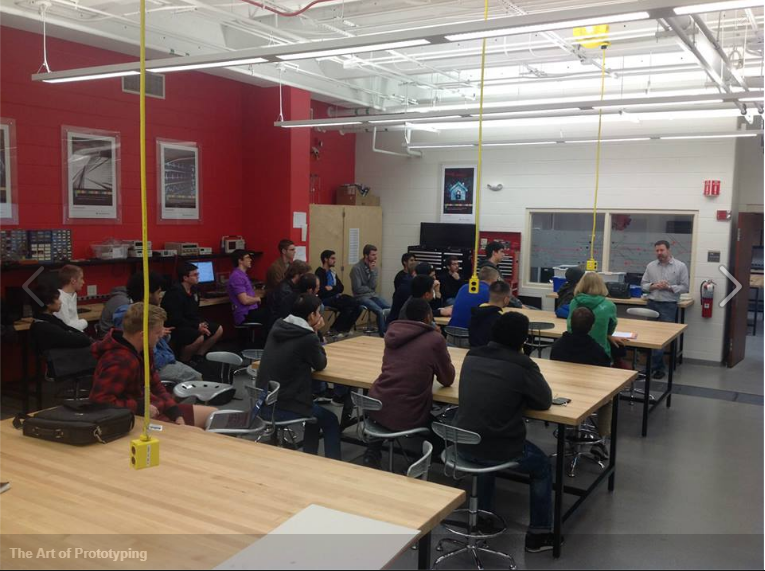
\includegraphics[width=0.7\textwidth, angle=0]{Workspaces/innovationlab.PNG}
  \caption{The UCF TI Innovation Lab, Courtesy of Mr. Harper}
 \end{figure}

\subsection*{Description}
The TI Innovation Lab, found in Engineering Building II in the University of Central Florida, is a makerspace directed by one of our mentors, Mr. Harper. It provides us access to large workshop with a wide range of tools and equipment, along with a soldering station and wiring for electrical needs as well as our most utilized resource, a laser cutter. This is where the team can cut new parts, build and assemble under the guidance of our mentor. We can also prototype and test here, as it allows us to think and modify as we wish. The team often meets here for unofficial meetings occasionally on weekdays and weekends. 

\textbf {\large UCF Machine Shop}
 \begin{figure}[h!]
 \centering
   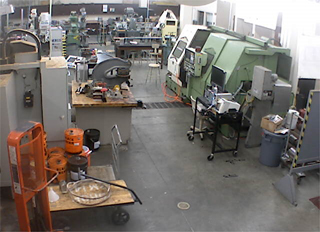
\includegraphics[width=0.7\textwidth, angle=0]{Workspaces/machine_shop.jpg}
  \caption{The UCF Machine Shop}
 \end{figure}

\subsection*{Description}
Right beside the TI Innovation Lab is the UCF Machine Shop, with heavy machinery like the lathe, the CNC Mill, drill press, and many more, all of which play a crucial role in making custom parts and pieces for our robot. With our mentor Mr. Harper also being a machinist, this is where the team learns from the best, using CAM tools to cut and create various pieces with ease. We use this machine shop throughout the season, whenever parts are required to be machined. This is a great workspace as it provides us with various resources that the team wouldn't even dream of having otherwise. It plays an essential role in our team's innovation and design. 